\documentclass[conference]{IEEEtran}

\usepackage{cite}
\usepackage{amsmath,amssymb,amsfonts}
\usepackage{verbatim} % um viele zeilen auszukommentieren
\usepackage{algorithmic}
\usepackage{graphicx}
\usepackage[ngerman]{babel}		% Achtung umlaut 
\usepackage[utf8]{inputenc}       % UTF-8 ist wichtig,  ASCII hat nicht alle Schriftzeichen  
\usepackage{textcomp}
\usepackage{xcolor}
\usepackage{dirtytalk} % nein, nicht was du denkst.  Packet hilft  gegen verschluckte gänsefüschen
\def\BibTeX{{\rm B\kern-.05em{\sc i\kern-.025em b}\kern-.08em
    T\kern-.1667em\lower.7ex\hbox{E}\kern-.125emX}}
\begin{document}

\title{Projekt rosBerry *\\
{\footnotesize \textsuperscript{*}Ein Autonomer Roboter auf der Basis von ROS , gebaut aus einem Modeauto Chassis mit Maker Elektronik}}

\author{\IEEEauthorblockN{1\textsuperscript{st} Welter, Heike}
\IEEEauthorblockA{\textit{Hochschule Mannheim} \\
email address 1630298@stud.hs-mannheim.de}%
\and
\IEEEauthorblockN{2\textsuperscript{nd} Matteis, Steffen}
\IEEEauthorblockA{\textit{Hochschule Mannheim} \\
email address}%noch 
\and
\IEEEauthorblockN{3\textsuperscript{rd}Barsalou Marie }
\IEEEauthorblockA{\textit{Hochschule Mannheim} \\
email address}
}

\maketitle

\begin{abstract}
Ziel von rosBerry besteht darin einen kleinen, schnellen aber dennoch preisgünstigen Roboter aus leicht verfügbaren Standartbauteilen zu Bauen. Zusätzlich soll er mit dem Robot Operating System Betrieben werden und mit einer Künstlichen Intelligenz versehen. Der Roboter soll einen optischen Marker erkennen und darauf zufahren. Frontal zusammenstöße mit Wänden soll er dabei Vermeiden. 
\end{abstract}

\begin{IEEEkeywords}
Roboter, ROS, KI, Raspi, Neuronale Netze, Arduiono
\end{IEEEkeywords}

%\section{Einleitung }  wollen wir  eine machen?
%projekteinleitung text hier
\section{Theorie zu dem Roboter und seiner Künstlichen Intelligenz}

\subsection{Vergleichbare Projekte}	%mary
Wenige Projekt der Robotik oder der Künstlichen Intelligenz für Autonome Systeme  existieren ohne das es nicht andere Vergleichbare Projekte gibt. \\


\subsubsection{Vergleichbare Hardware Ansätze Donkey Cars} %may
%Donkey car infos
Die Hardware des Roboters wurde vom Donkey car Projekt inspieriert. Das Donkey Car Projekt Beschäftigt sich damit ein Ferngesteuertes Auto mit einem Raspberry Pie zu steuern. Mehr Informationen zu dem Projekt gibt es auf ihrer Website. https://docs.donkeycar.com.  Donkey Cars Fahren größtenteils mit Hilfe von quelloffenem Python Code. \\
\\
Auf Youtube hat ein Benutzer namens "` Tiziano Fiorenzani"' gezeigt wie ein Donkey car mit ROS betrieben werden kann. Das Video https://youtu.be/iLiI\_IRedhI verweist auf Github für Tiziano Fiorenzanis code. Das Projekt wurde um einen Arduino und mehrere ROS Nodes erweitert.
% Tiziano der Rasende Italiener auf youtube
\subsubsection{Vergleichbare Projekte zur Künstlichen Intelligenz} %steffen ? mary?

 Das Neuronale Netz zur Bildklassifizierung ist an das Buch  Artificial Intelligence for Robotics  \cite{b1} angelehnt. Darin Vermittelt ein F. Grovers wie Künstliche Intelligenz für Autonome Systeme  funktionieren kann, in dem er zeigt wie er einem Kleine Roboter beibringen würde aufzuräumen. In Einem Kapitel Beschreibt der Autor das der Roboter mit Hilfe von Neuronalen Netzen lernen soll ob sich Spielzeuge auf dem Teppich befinden, um sie später aufzuräumen.  Da unsere Anwendungsfall ein anderer ist  musste die Datenmenge erhöht werden, das Neuronale Netz wurde erweitert und die Auflösung des Bildes wurde erhöht.\\

Auch die Bachelorarbeit  "`Bildklassifikation auf einem Raspberry Pi Zero
am Beispiel einer Ladestationserkennung"'  von Amanda Decker ist ein Vergleichbares Projekt.  Einige der Grundansätze wie  dieser Arbeit wurden für dieses Projekt übernommen. So haben wir das Neuronale Netz nicht auf einem Raspberry Pie Trainiert und einen Marker genommen der sich gut rotieren und Spiegeln lässt. So kann Jedes Bild des Datensatzes gespiegelt werden um mit mehr Daten arbeiten zu können. Anders als Amanda Decker jedoch haben wir uns für Keras entschieden, statt eine selbstgeschriebene Künstliche Intelligenz zu verwenden. 
\section{Theoretische Grundlagen von Projekt rosBerry}

\subsection{Neuronale Netze in Theorie}	%steffen

\subsection{Ansätze für die Erstellung vom Datensatz}	%mary

Bei Amanda Dekers Bachelorarbeit schien die KI Schwierigkeiten damit zu haben zwischen  dem Marker und einem Blauton zu unterscheiden der auch im Marker vorkam. Es schien auch schwierig zu sein ein Binärbild von dem Marker zu erzeugen, da die beiden Farben des Marker einen geringen Kontrast zueinander haben. Da Kameras in Opencv mit Hilfe von Schachbrettmustern kalibriert werden, wird für dieses Projekt ein Symbol mit ähnlich Hohem Kontrast und Schafen Kanten verwendet.\\
%Marker Bild hier?
 Dieses Symbol ist nicht nur in 4 Richtungen Rottierbar sondern auch zweifach Spiegelbar ohne den Marker zu verfälschen. (Rotations invariant und spiegelungs invariant.) Es verfügt auch über einen Maximalen Kontrast und klare, gerade Kannten. \\
 \noindent
Ein Neuronales Netz kann nur so gut sein wie die Daten mit denen es trainiert und getestet wurde. In vielen wissenschaftlichen und Populärwissenschaftlichen Artikeln wurde beschrieben wie ein ungeeigneter Datensatz zu unbrauchbaren Ergebnissen führte. So wurden die verurteile der Forscher bestätigt, oder die KI traf Entscheidungen anhand von den Flaschen Kriterien, wie der Bildunterschrift statt dem Bildinhalt. \\
Um einen Möglichst Robusten Datensatz zu bekommen  werden verschiedene Techniken angewendet.
\begin{itemize}
	\item Um zu verhindern das die KI alle Bilder mit starken Kontrasten für einen Marker hält wird ein Auschnitt einmal mit und ein mal ohne den Marker Fotografiert.
	\item Gegen den  "`schön-wetter KI"' Effekt (eine KI die annimmt jedes gut ausgeleuchtete Bild muss ein Treffer sein) wird der Marker bei verschiedenen Beleuchtungen Fotografiert. Dazu gehören Direktes Sonnenlicht, Schatten, Künstliche Beleuchtung mit LED Lampen und Neon Röhren. 
	\item Um zu verhindern das die KI alles für ihren Marker hält, was eine gewisse gösse hat und quadratisch ist, wurde der Marker aus verschiedenen Distanzen Fotografiert. 
	\item Gegen Noise Anfälligkeit wurden verschiedene Hintergründe bei den Fotos verwendet. Teils weiße wände teils strukturierte Hintergründe oder eine Freifläche. 
	\item Um zu verhindern das sich die KI auf die Bildmitte Konzentrieren kann wird der Marker aus verschieden Positionen Fotografiert. 
\end{itemize}

% bilder ++
% wie unterschiedliche bilder
\subsection{ROS Knoten Software Architektur}%heike
%grobstruktur,  nodes topics und all das was es schon als text gibt
\subsubsection{ Launch Reihenfolge}%heike

\section{Praktische Projekt Durchführung }

\subsection{Hardware aufbau}%Heike 


\section{Autonomes verhalten durch Künstliche Intelligenz  }	%mary
%was machen wir da eigentlich
%was ist unser ziel
%wiso haben wir uns dafür entschiden

\subsection{Erster Ansatz für das Neuronale Netz}	%steffen ? mary?
%netzaufbau am anfang
\subsubsection{Este Auswertung der Ergebnisse}	%steffen? 
%wiso war das scheisse
\subsection{Schritte zur Verbesserungen der Erkennungsrate} %mary
%was haben wir dann gemacht 
\subsection{Anwendung des Trainingsmodells } %steffen +mary
%bild teilen
%bild analysieren
%  entscheidung treffen, rechts, links geradeaus oder rückwärtz
\subsection {Auswertung des verhalten des Roboters}	% mary? %steffen? %heike?
%macht er irgendwas sinnvolles? ist er klüger als eine eintagsfliege

\begin{comment}	%  how-to formeln 
\begin{equation}
a+b=\gamma\label{eq}
\end{equation}
\end{comment}
\begin{comment}
\paragraph{Positioning Figures and Tables} 
 Use the abbreviation 
``Fig.~\ref{fig}'', even at the beginning of a sentence.

\begin{table}[htbp]
\caption{Table Type Styles}
\begin{center}
\begin{tabular}{|c|c|c|c|}
\hline
\textbf{Table}&\multicolumn{3}{|c|}{\textbf{Table Column Head}} \\
\cline{2-4} 
\textbf{Head} & \textbf{\textit{Table column subhead}}& \textbf{\textit{Subhead}}& \textbf{\textit{Subhead}} \\
\hline
copy& More table copy$^{\mathrm{a}}$& &  \\
\hline
\multicolumn{4}{l}{$^{\mathrm{a}}$Sample of a Table footnote.}
\end{tabular}
\label{tab1}
\end{center}
\end{table}

\begin{figure}[htbp]
\centerline{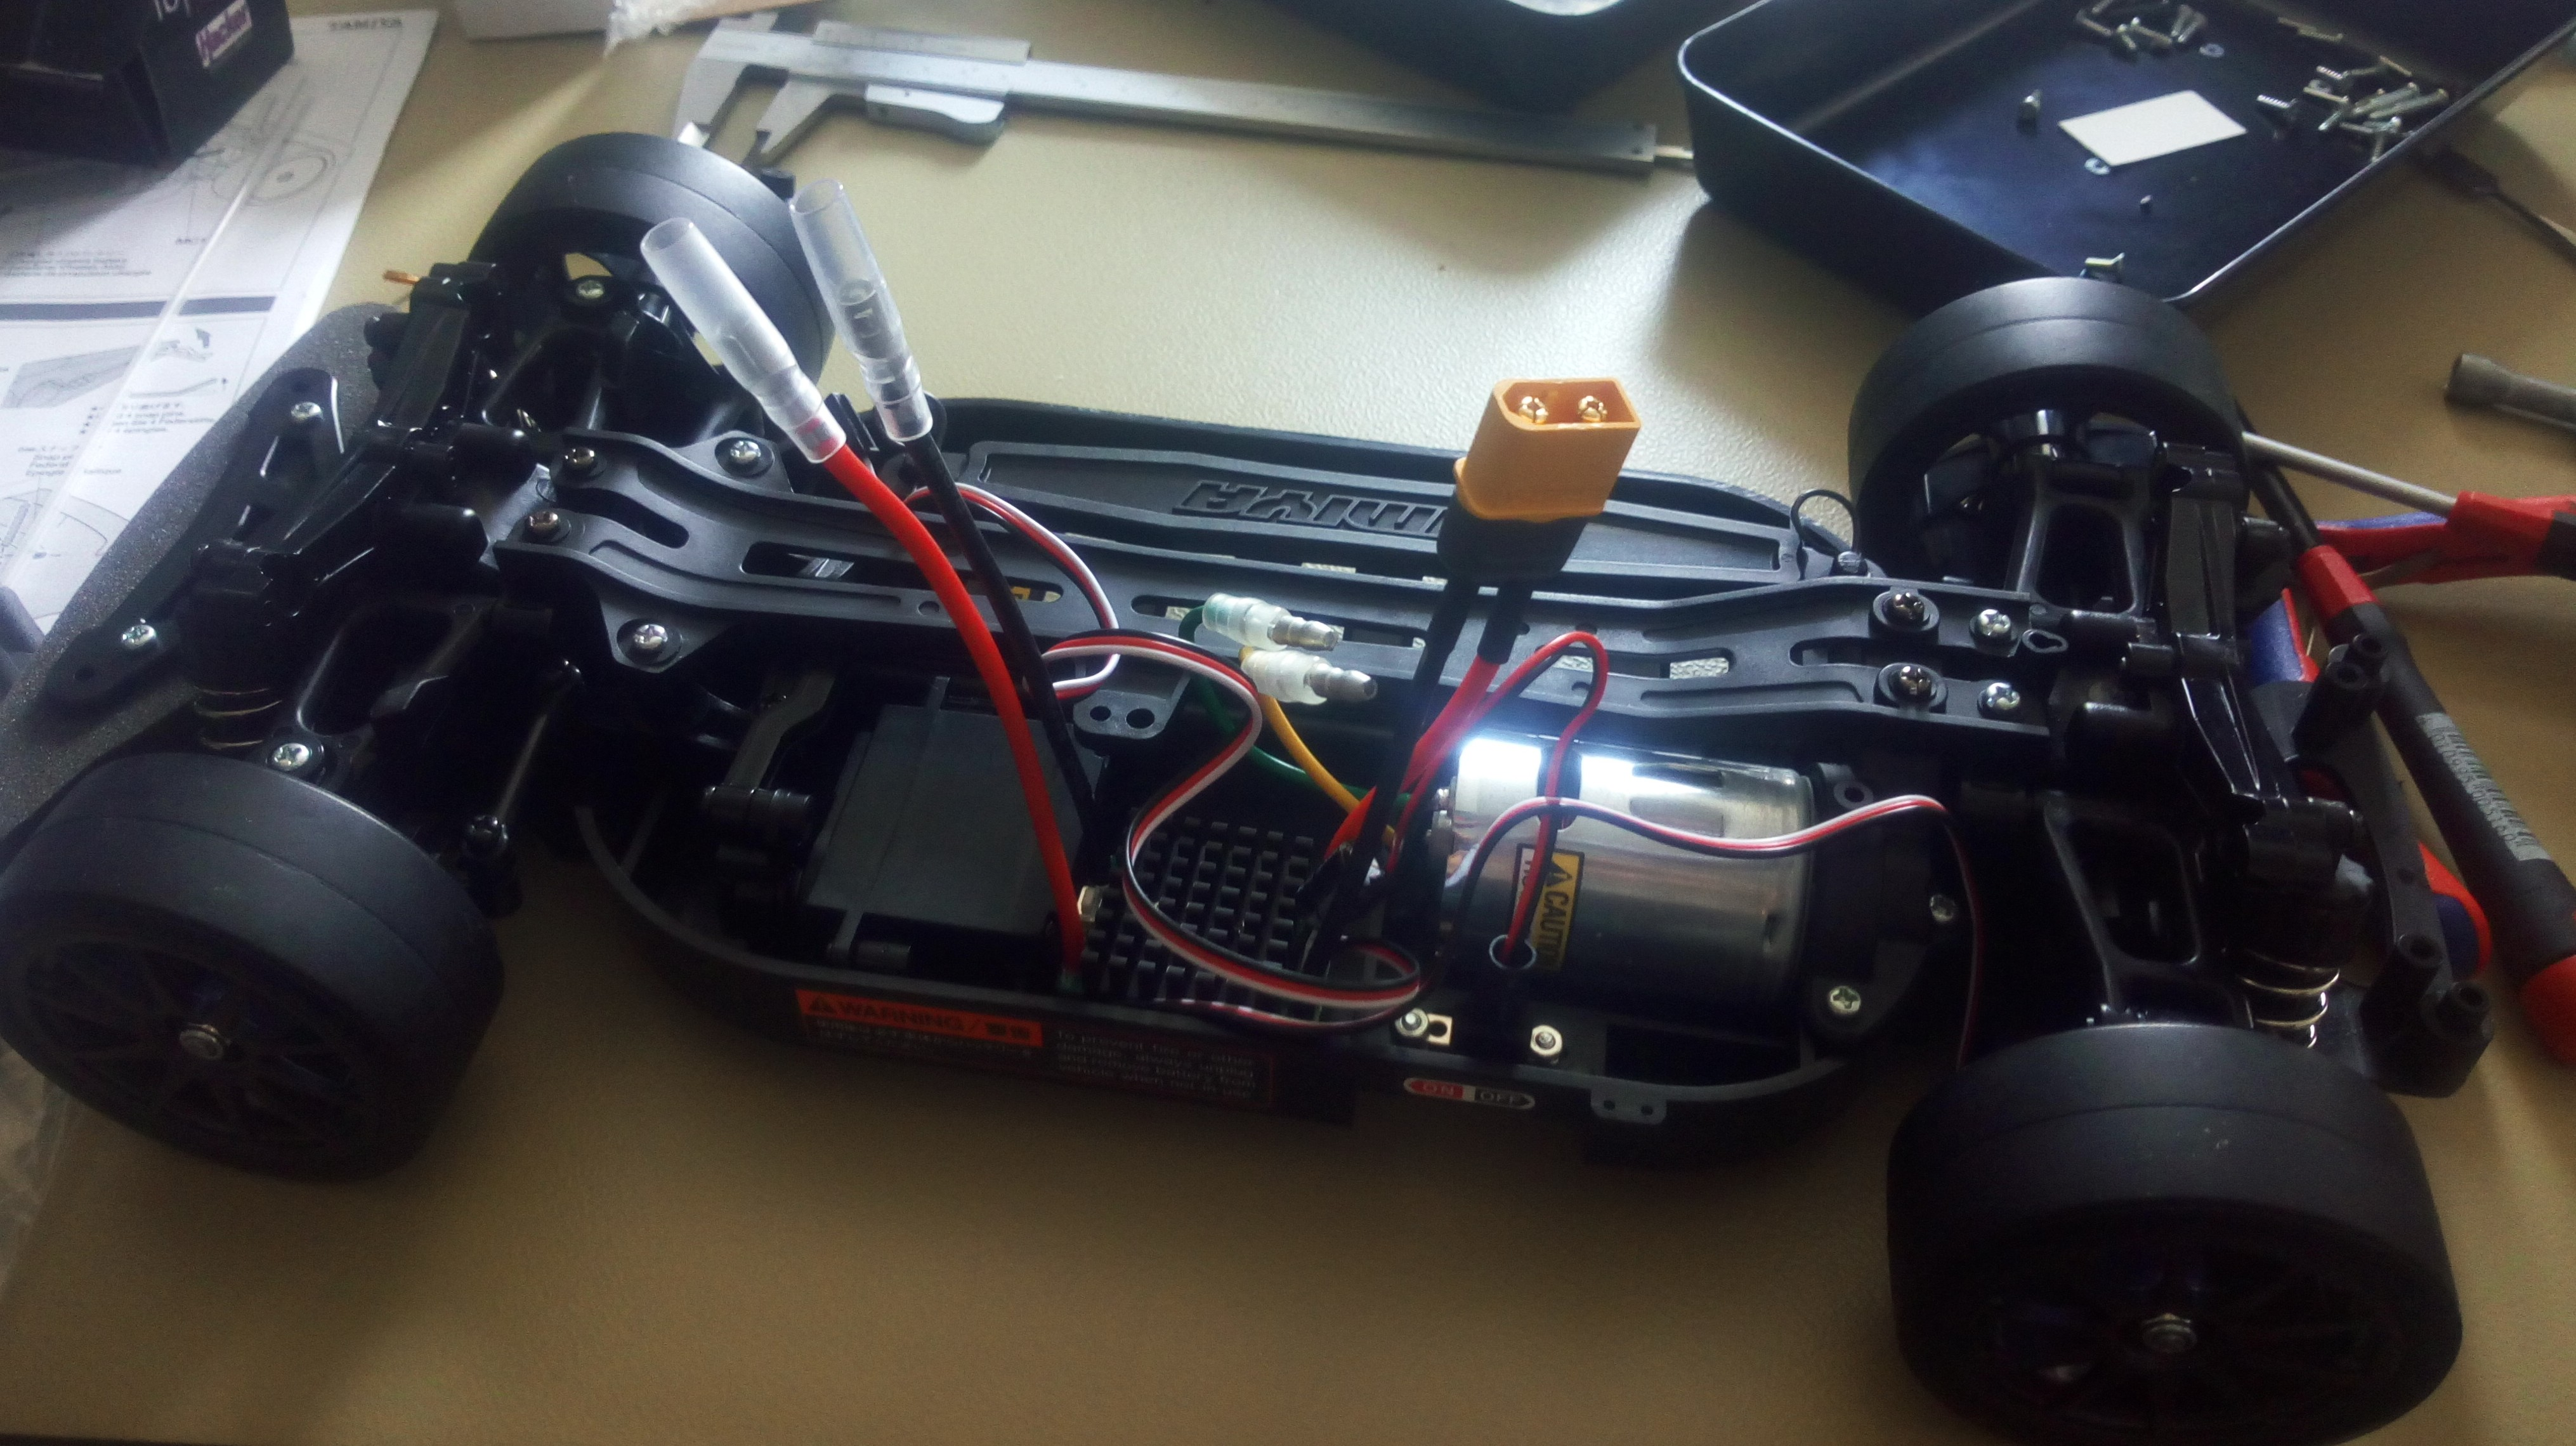
\includegraphics{img/car_body.jpg}}
\caption{Example of a figure caption.}
\label{fig}
\end{figure}
\end{comment}


%\section*{Acknowledgment}
% wollen wir unseren profs danken, weil mehr GPU und RAM? 

% wissenschaftliche zitate gehen so \cite{b1}. 


%Francis X. Govers - Artificial Intelligence for Robotics-Packt Publishing (2018).pdf
\begin{thebibliography}{00}
\bibitem{b1}Francis X. Govers , ` Artificial Intelligence for Robotics,''Packt Publishing ,2018

\end{thebibliography}


\end{document}
